\documentclass{article}
\usepackage{amsfonts, amsmath, amssymb, amsthm, dsfont} % Math notations imported
\usepackage{enumitem}
\usepackage{graphicx}
\usepackage{setspace}
\usepackage{indentfirst}
\usepackage[margin=1in]{geometry}
\graphicspath{{./images/}} % Path to images

% \begin{figure}[htb!]
%      \centering
%      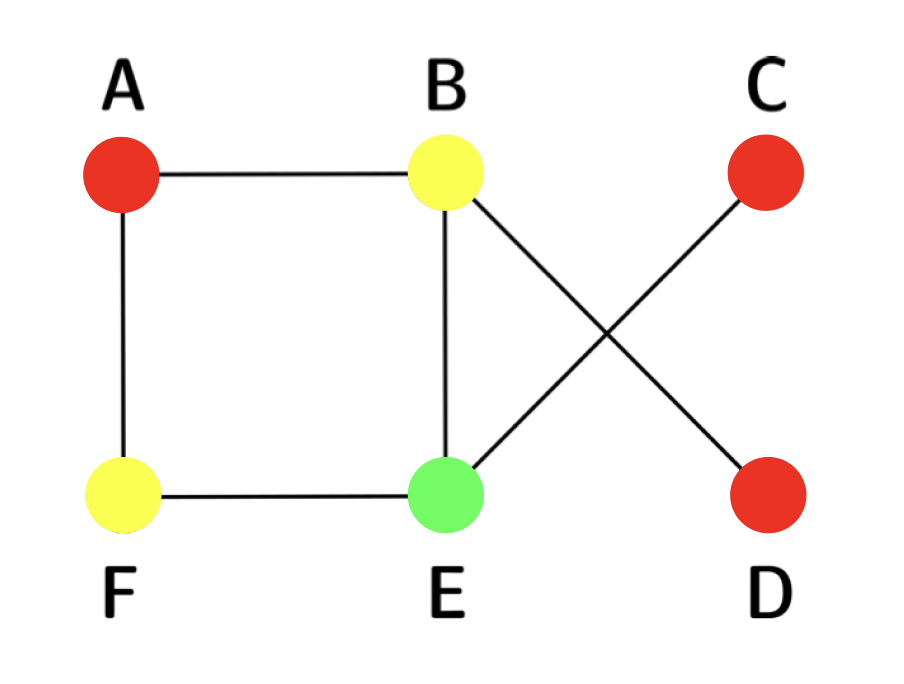
\includegraphics[scale=0.5]{coloring.png}
%      \caption{Coloring of the graph.}
% \end{figure}

% \begin{figure}[htb]
%     \qquad
%     \begin{minipage}{.4\textwidth}
%         \centering
%         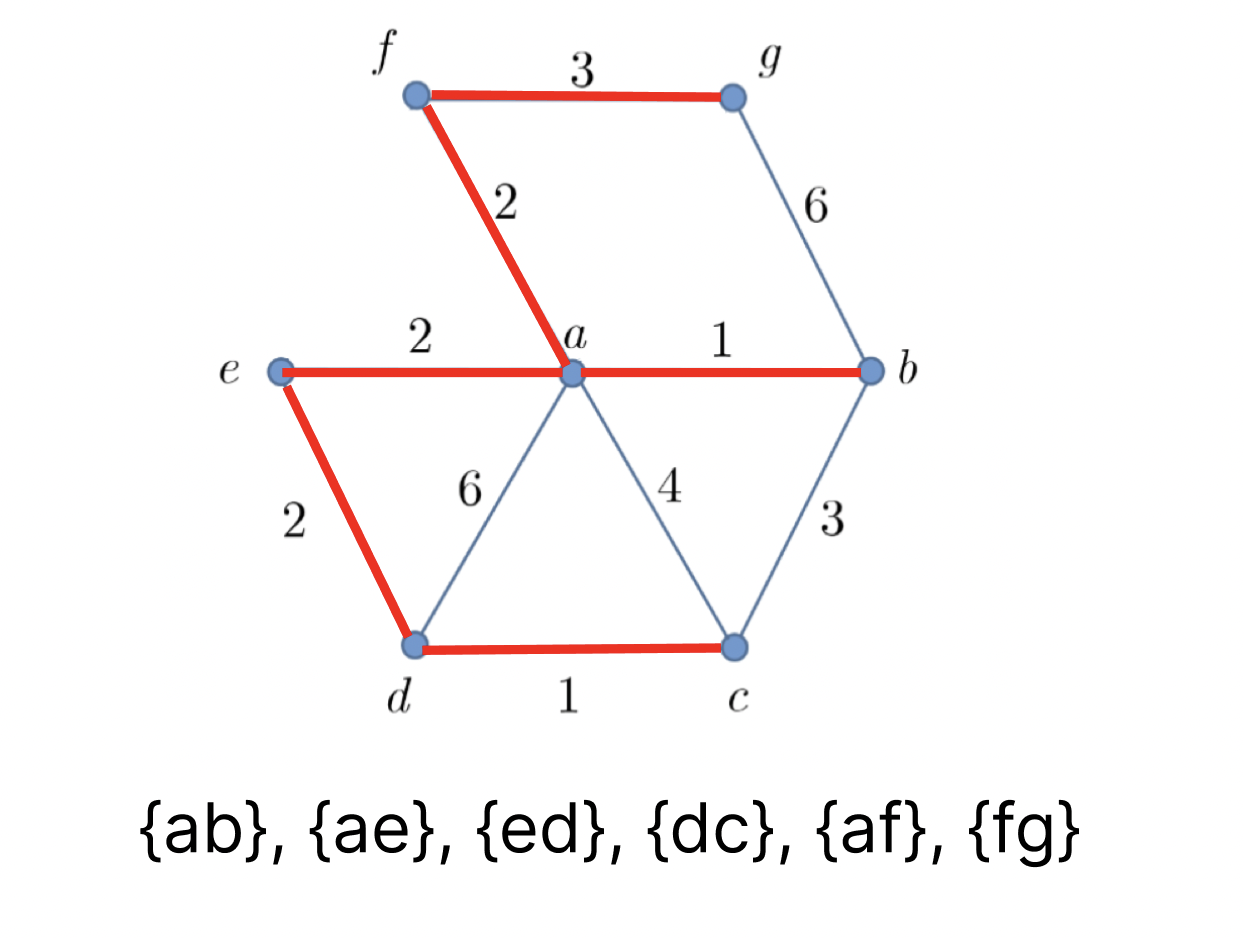
\includegraphics[scale=0.35]{prims.png}
%         \caption{}
%     \end{minipage}    
%     \qquad
%     \begin{minipage}{.4\textwidth}
%         \centering
%         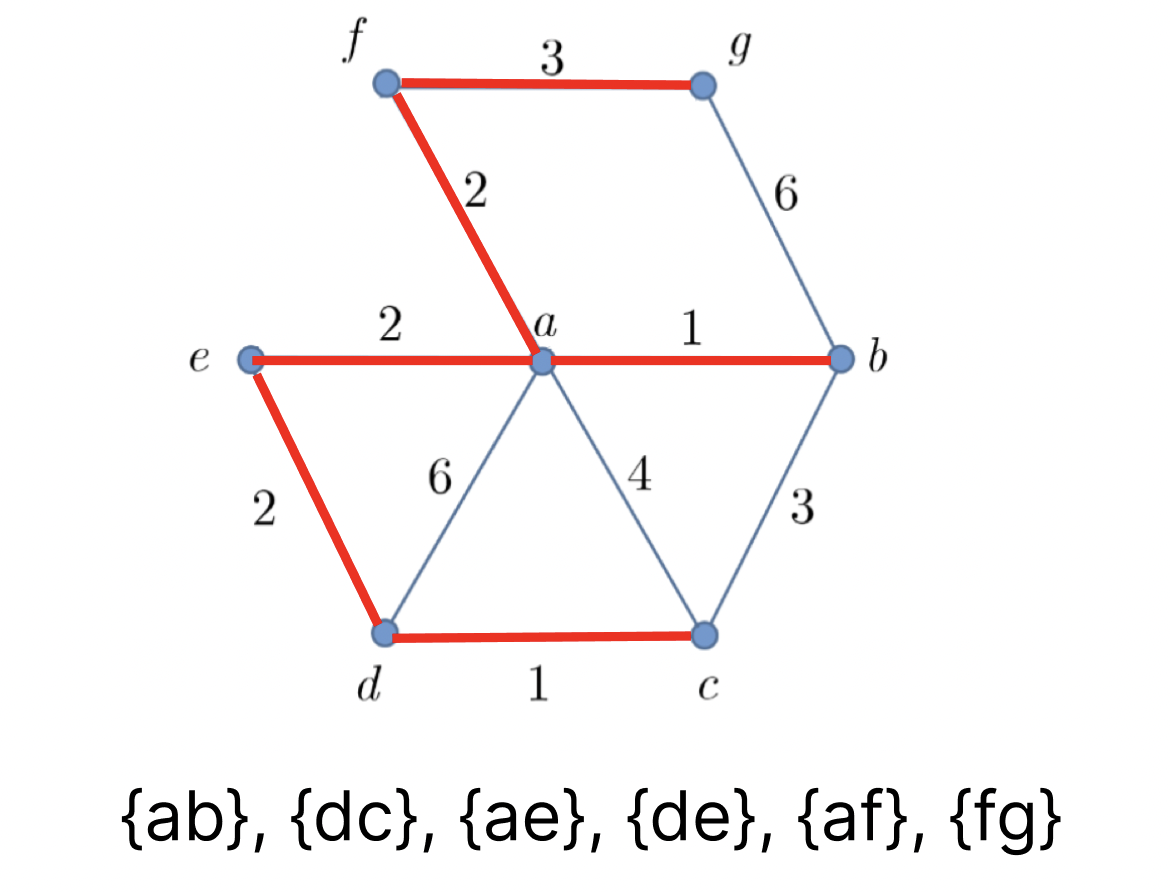
\includegraphics[scale=0.35]{kruskal.png}
%         \caption{}
%     \end{minipage}        
% \end{figure} 

\newtheorem{thm}{Theorem}
\newtheorem{proposition}[thm]{Proposition}
\newtheorem{corollary}[thm]{Corollary}
\newtheorem{lemma}[thm]{Lemma}

\newcommand*{\Var}{\ensuremath{\mathrm{Var}}}
\newcommand*{\Cov}{\ensuremath{\mathrm{Cov}}}
\newcommand*{\Corr}{\ensuremath{\mathrm{Corr}}}
\newcommand*{\Bias}{\ensuremath{\mathrm{Bias}}}
\newcommand*{\MSE}{\ensuremath{\mathrm{MSE}}}
\newcommand*{\range}{\ensuremath{\mathrm{range}}\,}
\newcommand*{\spann}{\ensuremath{\mathrm{span}}\,}
\newcommand*{\nul}{\ensuremath{\mathrm{null}}\,}
\newcommand*{\dom}{\ensuremath{\mathrm{dom}}\,}
\renewcommand*{\implies}{\ensuremath{\Longrightarrow}}
\renewcommand*{\impliedby}{\ensuremath{\Longleftarrow}}
\newcommand*{\Z}{\ensuremath{\mathbb{Z}}}
\newcommand*{\Q}{\ensuremath{\mathbb{Q}}}
\newcommand*{\R}{\ensuremath{\mathbb{R}}}
\newcommand*{\F}{\ensuremath{\mathbb{F}}}
\newcommand*{\C}{\ensuremath{\mathbb{C}}}
\newcommand*{\N}{\ensuremath{\mathbb{N}}}
\newcommand*{\E}{\ensuremath{\mathds{E}}}
\renewcommand*{\P}{\ensuremath{\mathds{P}}}
\newcommand*{\p}{\ensuremath{\mathcal{P}}}

% title information
\title{Math 104 HW11}
\author{Neo Lee}
\date{11/24/2023}

\setstretch{1.15}
% main content
\begin{document} 

% placing title information; comment out if using fancyhdr
\maketitle 

\subsection*{Exercise 29.2}
\begin{proposition}
    $|\cos x-\cos y|\le |x-y|$ for all $x,y\in\R$.
\end{proposition}
\begin{proof}
    Notice that the inequality looks similar to the slope of the function $\cos x$ evaluated 
    on the interval $[x,y]$.

    Since $\cos x$ is continuous and differentiable on $\R$, by mean value value theorem, 
    there exists $c\in(x,y)$ such that
    \begin{align*}
        \frac{\cos x - \cos y}{x-y} & = \cos'(c) \\
        \frac{\cos x - \cos y}{x-y} & = -\sin(c).
    \end{align*}
    Then notice that $|\sin(c)|\le 1$ for all $c\in\R$, so we have for all $x,y\in\R$,
    \begin{align*}
        \left|\frac{\cos x - \cos y}{x-y}\right| & = |\sin(c)| \\
        \left|\frac{\cos x - \cos y}{x-y}\right| & \le 1 \\
        |\cos x - \cos y| & \le |x-y|.
    \end{align*}
\end{proof}

\newpage
\subsection*{Exercise 29.5}
\begin{proposition}
    Let $f$ be defined on \R, and suppose $|f(x)-f(y)|\le(x-y)^2$ for all $x,y\in\R$, 
    then $f$ is a constant function.
\end{proposition}
\begin{proof}
    Fix arbitrary $y\in\R$, then we have for all $x\in\R$,
    \begin{align*}
        |f(x)-f(y)| & \le (x-y)^2 \\
        \left|\frac{f(x)-f(y)}{x-y}\right| & \le |x-y|.
    \end{align*}
    Since $\lim_{x\to y}|x-y| = 0$, for all $\epsilon>0$, there exists $\delta>0$ such that
    $|x-y|<\delta$ implies $|x-y|<\epsilon$. Then we have for all $x\in\R$ such that 
    $|x-y|<\delta$, 
    $$\left|\frac{f(x)-f(y)}{x-y}\right| \le |x-y|<\epsilon,$$
    and $$\lim_{x\to y}\left|\frac{f(x)-f(y)}{x-y}\right|=0.$$
    Then by definition of derivative, we have $f'(y)=0$. Since $y$ is arbitrary,
    we have $f'(x)=0$ for all $x\in\R$. Then by \emph{Corollary 29.4}, we have $f$ is a constant
    function.
\end{proof}


\newpage
\subsection*{Exercise 29.11}
\begin{proposition}
    $\sin x \le x$ for all $x\ge 0$.
\end{proposition}
\begin{proof}
    Notice $x-\sin x$ is differentiable on $[0,\infty)$ because both $x$ and $\sin x$ are
    differentiable on $[0,\infty)$. Then we have for all $x\ge 0$,
    \begin{align*}
        (x-\sin x)' & = 1-\cos x \\
        (x-\sin x)' & = 1-\cos x \ge 0.
    \end{align*}
    Then by \emph{Corollary 29.7}, we have $x-\sin x$ is increasing on $[0,\infty)$, so
    for $x\ge0$, we have $x-\sin x\ge 0$ because $x-\sin x = 0$ for $x=0$. Then we have
    for all $x\ge 0$, $\sin x \le x$.
\end{proof}

\newpage
\subsection*{Exercise 29.18}
\begin{proposition}
    Let $f$ be differentiable on $\R$ with $a=\sup\{|f'(x):x\in\R|\}<1$.
    \begin{enumerate}[label=\textbf{(\alph*)}]
        \item Select $s_0\in\R$ and define $s_n=f(s_{n-1})$ for $n\ge 1$. Thus $s_1=f(s_0)$,
        $s_2=f(s_1)$, etc. Then $(s_n)$ is a convergent sequence.

        \item $f$ has a fixed point, i.e., $f(s)=s$ for some $s\in\R$.
    \end{enumerate}
\end{proposition}
\begin{proof}
    \begin{enumerate}[label=\textbf{(\alph*)}]
        \item 
        Since $f$ is differentiable and hence continuous on $\R$, there exists $c$ between $s_n$ and $s_{n-1}$
        such that 
        $$\frac{f(s_n) - f(s_{n-1})}{s_n-s_{n-1}} = f'(c).$$
        Then, since $|f'(c)|\le a<1$, we have for all $n\in\N$,
        $$|s_{n+1}-s_n| = |f(s_n) - f(s_{n-1})| = |f'(c)||s_n-s_{n-1}| \le a|s_n-s_{n-1}|.$$
        In particular, $|s_{n+1}-s_n|\le a^n|(s_1-s_0)|.$ Therefore, without loss of generality, for some $n> m \in\N$, 
        \begin{align*}
            |s_n-s_m| & = |(s_n - s_{n-1}) + (s_{n-1} - s_{n-1})\cdots + (s_{m+1}-s_m)| \\
            |s_n-s_m| & \le |s_n-s_{n-1}| + |s_{n-1} - s_{n-1}|\cdots + |s_{m+1}-s_m| \\
            |s_n-s_m| & \le a^{n-1}|(s_1-s_0)| + a^{n-2}|(s_1-s_0)|\cdots + a^m|(s_1-s_0)| \\
            |s_n-s_m| & \le |(s_1-s_0)|\sum_{k=m}^{n-1}a^k \\
            |s_n-s_m| & \le \lim_{n\to\infty}|(s_1-s_0)|\sum_{k=m}^{n-1}a^k = a^m\frac{|(s_1-s_0)|}{1-a}.
        \end{align*}
        Now notice $$\lim_{m\to\infty}a^m\frac{|(s_1-s_0)|}{1-a} = 0,$$
        so there exists $N\in\N$ such that for all $m> N$, 
        $$a^m\frac{|(s_1-s_0)|}{1-a} < \epsilon,$$
        therefore, for all $n\ge m>N$,
        $$|s_n-s_m| < \epsilon.$$
        Then $(s_n)$ is a Cauchy sequence hence a convergent sequence.

        \item 
        Since $(s_n)$ is a convergent sequence, there exists $s\in\R$ such that
        $$\lim_{n\to\infty}s_n = s.$$
        Then since $f$ is continuous, we have
        $$\lim_{n\to\infty}f(s_n) = f(s).$$
        Now recall that $s_{n+1}=f(s_n)$ for all $n\ge 1$, so we have
        $$s = \lim_{n\to\infty}s_{n+1} = \lim_{n\to\infty}f(s_n) = f(s).$$
    \end{enumerate}
\end{proof}


\newpage
\subsection*{Exercise 30.2}
Find the following limits if they exist,
\begin{enumerate}[label=\textbf{(\alph*)}]
    \item $\lim_{x\to0}\frac{x^3}{\sin x -x}$
    \item $\lim_{x\to0}\frac{\tan x - x}{x^3}$
    \item $\lim_{x\to0}\left(\frac{1}{\sin x}-\frac{1}{x}\right)$
    \item $\lim_{x\to0}(\cos x)^{1/x^2}$
\end{enumerate}
\begin{proof}[Solution]\indent
    \begin{enumerate}[label=\textbf{(\alph*)}]
        \item \begin{align*}
            \lim_{x\to0}\frac{x^3}{\sin x -x} & = \lim_{x\to0}\frac{3x^2}{\cos x -1} \\
            & = \lim_{x\to0}\frac{6x}{-\sin x} \\
            & = \lim_{x\to0}\frac{6}{-\cos x} \\
            & = -6.
        \end{align*}

        \item \begin{align*}
            \lim_{x\to0}\frac{\tan x - x}{x^3} & = \lim_{x\to0}\frac{\sec^2 x - 1}{3x^2} \\
            & = \lim_{x\to0}\frac{2\sec^2 x\tan x}{6x} \\
            & = \lim_{x\to0}\frac{-4\sec^2 x + 6\sec^4 x}{6} \\
            & = \frac{1}{3}.
        \end{align*}

        \item
        \begin{align*}
            \lim_{x\to0}\left(\frac{1}{\sin x}-\frac{1}{x}\right) & = \lim_{x\to0}\frac{x-\sin x}{x\sin x} \\
            & = \lim_{x\to0}\frac{1-\cos x}{\sin x + x\cos x} \\
            & = \lim_{x\to0}\frac{\sin x}{2\cos x -x\sin x} \\
            & = 0.
        \end{align*}

        \item 
        $$\lim_{x\to0}\lim_{x\to0}(\cos x)^{1/x^2} = \lim_{x\to0}e^{\ln(\cos x)/x^2}.$$
        Now, \begin{align*}
            \lim_{x_to0}\frac{\ln(\cos x)}{x^2} & = \lim_{x\to0}\frac{-\tan x}{2x} \\
            & = \lim_{x\to0}\frac{-\sec^2 x}{2} \\
            & = -\frac{1}{2}.
        \end{align*}
        Since $e^x$ is continuous, we have
        $$\lim_{x\to0}\lim_{x\to0}(\cos x)^{1/x^2} = \lim_{x\to0}e^{\ln(\cos x)/x^2} = e^{-1/2}.$$
    \end{enumerate}    
\end{proof}


\newpage
\subsection*{Exercise 30.5}
Find the limits
\begin{enumerate}[label=\textbf{(\alph*)}]
    \item $\lim_{x\to0}(1+2x)^{1/x}$
    \item $\lim_{y\to\infty}(1+\frac{2}{y})^y$
    \item $\lim_{x\to\infty}(e^x+x)^{1/x}$
\end{enumerate}
\begin{proof}[Solution]\indent
    \begin{enumerate}[label=\textbf{(\alph*)}]
        \item 
        $$\lim_{x\to0}(1+2x)^{1/x} = \lim_{x\to0}e^{\ln(1+2x)/x}.$$
        Now \begin{align*}
            \lim_{x\to0}\frac{\ln(1+2x)}{x} & = \lim_{x\to0}\frac{2}{1+2x} \\
            & = 2.
        \end{align*}
        Since $e^x$ is continuous, we have
        $$\lim_{x\to0}(1+2x)^{1/x} = \lim_{x\to0}e^{\ln(1+2x)/x} = e^2.$$

        \item
        $$\lim_{y\to\infty}(1+\frac{2}{y})^y = \lim_{y\to\infty}e^{y\ln(1+\frac{2}{y})}.$$
        Now, 
        \begin{align*}
            \lim_{y\to\infty}y\ln(1+\frac{2}{y}) & = \lim_{y\to\infty}\frac{\ln(1+\frac{2}{y})}{\frac{1}{y}} \\
            & = \lim_{y\to\infty}\frac{\frac{-2}{y^2(1+2/y)}}{\frac{-1}{y^2}} \\
            & = \lim_{y\to\infty}\frac{2}{1+2/y} \\
            & = 2.
        \end{align*}
        Since $e^x$ is continuous, we have
        $$\lim_{y\to\infty}(1+\frac{2}{y})^y = \lim_{y\to\infty}e^{y\ln(1+\frac{2}{y})} = e^2.$$

        \item
        $$\lim_{x\to\infty}(e^x+x)^{1/x} = \lim_{x\to\infty}e^{\ln(e^x+x)/x}.$$
        Now,
        \begin{align*}
            \lim_{x\to\infty}\frac{\ln(e^x+x)}{x} & = \lim_{x\to\infty}\frac{e^x+1}{e^x+x} \\
            & = \lim_{x\to\infty}\frac{e^x}{e^x+x} + \lim_{x\to\infty}\frac{1}{e^x+x} \\
            & = \lim_{x\to\infty}\frac{e^x}{e^x+1} + 0 \\
            & = \lim_{x\to\infty}\frac{e^x}{e^x} \\
            & = 1.
        \end{align*}
        Since $e^x$ is continuous, we have
        $$\lim_{x\to\infty}(e^x+x)^{1/x} = \lim_{x\to\infty}e^{\ln(e^x+x)/x} = e^1 = e.$$
    \end{enumerate}
\end{proof}

\end{document}
